\documentclass[12pt]{article}

\title{Progetto di sistemi complessi}
\author{Simone Balducci, Alessandro Mancini}
\date{}

\usepackage{amsmath}
\usepackage{amsfonts}
\usepackage{amssymb}
\usepackage{amsthm}
\usepackage{braket}
\usepackage{bbold}
\usepackage[margin=2cm]{geometry}
\usepackage{pgfplots}
\usepackage{fancyhdr}
\usepackage{physics}
\usepackage{systeme,mathtools}
\usepackage{graphicx}
\graphicspath{{./}}
\usepackage{float}
\usepackage{relsize}
\usepackage{dsfont}
\usepackage{calligra}
%\usepackage{siunitx}


\newcommand{\vv}{\vec{v}}
\newcommand{\vw}{\vec{w}}
\newcommand{\vov}{\vec{0_V}}
\newcommand{\vow}{\vec{0_W}}
\newcommand{\vo}{\vec{0}}
\newcommand{\vx}{\vec{x}}
\newcommand{\R}{\Re}
\newcommand{\la}{\lambda}
\newcommand{\bd}{\textbf}
\newcommand{\lang}{\left\langle}
\newcommand{\rang}{\right\rangle}
\newcommand{\lbra}{\left\lbrace}
\newcommand{\rbra}{\right\rbrace}
\newcommand{\ih}{\hat{i}}
\newcommand{\jh}{\hat{j}}
\newcommand{\kh}{\hat{k}}
\newcommand{\nnabla}{\vec{\nabla}}
\newcommand{\vr}{\vec{r}}
\newcommand{\vac}{\vec{a}}
\newcommand{\vf}{\vec{F}}
\newcommand{\vp}{\vec{p}}
\newcommand{\vom}{\vec{\omega}}
\newcommand{\val}{\vec{\alpha}}
\newcommand{\vsr}{\vec{\mathlarger{\mathlarger{\mathlarger{\scriptr}}}}}
\makeatletter
\newcommand*\bigcdot{\mathpalette\bigcdot@{.5}}
\newcommand*\bigcdot@[2]{\mathbin{\vcenter{\hbox{\scalebox{#2}{$\m@th#1\bullet$}}}}}
\makeatother
\def\dbar{{\mathchar'26\mkern-12mu d}}
\DeclareMathAlphabet{\mathcalligra}{T1}{calligra}{m}{n}
\DeclareFontShape{T1}{calligra}{m}{n}{<->s*[2.2]callig15}{}
\newcommand{\scriptr}{\mathcalligra{r}\,}
\newcommand{\boldscriptr}{\pmb{\mathcalligra{r}}\,}

\begin{document}

\maketitle 
\section{L'oscillatore di Van Der Pol}
\subsection{Descrizione}
L'oscillatore di Van Der Pol è un sistema dinamico composto da un oscillatore smorzato, descritto dalla seguente equazione:
\begin{equation}
	\ddot{x} - \mu(1-x^2)\dot{x} + x = 0
\end{equation}
dove $x(t)$ indica l'oscillazione nello spazio delle configurazioni in funzione del tempo e $\mu$ è una costante che indica lo smorzamento. Il termine di mezzo dell'equazione è quello responsabile dello smorzamento, e quindi dell'attrito. 
\begin{figure}[h]
	\begin{center}
		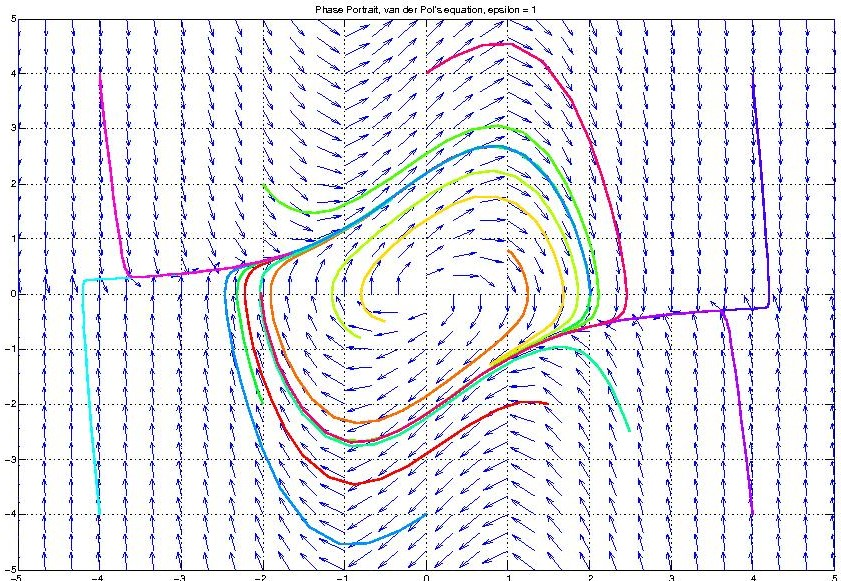
\includegraphics[scale=.5]{Spazio delle fasi oscillatore} 
		\caption{Questa figura mostra traiettorie caratteristiche dell'oscillatore di Van Der Pol nello spazio delle fasi per vari punti iniziali. Si noti anche che l'orientamento del campo vettoriale indirizza tutti i punti materiali verso la stessa traiettoria limite.}
	\end{center}
\end{figure}
Si nota subito che nel caso in cui la costante di smorzamento $\mu$ abbia valore nullo, si ottiene un oscillatore armonico classico, e questo verrà verificato nelle sezioni successive mediante simulazioni al computer e esperimenti mediante circuiti elettronici. 
\paragraph{Studio dell'equazione differenziale \\}
Consideriamo l'equazione (1) e riscriviamola come:
\begin{equation}
	\ddot{x}+\mu(x^2-1)\dot{x} = \frac{d}{dt}\left(\dot{x}+\mu\left(\frac{1}{3}x^3-x\right)\right) = \frac{d}{dt}\left(\dot{x} + \mu F(x)\right)
\end{equation}
definiamo quindi una nuova variabile
\begin{equation}
	w = \dot{x} + \mu F(x)
\end{equation}
avente derivata 
$$
	\dot{w} = -x
$$
Si ottiene quindi il sistema di equazioni
\begin{equation}
	\begin{cases}
		\dot{x} = w - \mu F(x) \\
		\dot{w} = -x
	\end{cases}
\end{equation}
Studiamo il caso $\dot{x} = 0$, che risulta in
\begin{equation}
	w(x) = \mu F(x) = \mu\left(\frac{1}{3}x^3-x\right)
\end{equation}
e si ottiene quindi una cubica. Studiamo quindi il grafico di questa funzione: 
\begin{center}
\begin{tikzpicture}
\begin{axis}[
	axis y line = center,
	axis x line = middle,
	xlabel = \( x \),
	ylabel = \( w \),
	width = 14cm,
	height = 10cm,
]
\addplot[
	domain = -2.5:2.5,
	samples = 150,
	color = black,
] {(1/3)*x^3-x};
\addplot[mark=*] coordinates {(2,2/3)} node[pin={$A$}]{};
\addplot[mark=*] coordinates {(-2,-2/3)} node[pin=180:{$C$}]{};
\addplot[mark=*] coordinates {(-1,2/3)} node[pin={$D$}]{};
\addplot[mark=*] coordinates {(1,-2/3)} node[pin=270:{$B$}]{};
\end{axis};
\end{tikzpicture}
\end{center}
Vediamo che $\dot{w} = 0$ solo per $x=0$, ovvero quando siamo sull'asse delle $y$, e si trova in particolare che sopra l'asse delle $x$ i vettori del campo vettoriale puntano a destra, mentre sotto l'asse delle $x$ puntano a sinistra. Il punto di massimo locale della funzione è $\left(-1,\frac{2}{3}\mu\right)$, mentre il punto di minimo locale è $\left(1,-\frac{2}{3}\mu\right)$. In più vediamo che i punti di intersezione tra le orizzontali che passano per i punti di massimo e minimo con la curva $w$ sono rispettivamente $\left(2,\frac{2}{3}\mu\right)$ $\left(-2,-\frac{2}{3}\mu\right)$. \\
Se consideriamo valori di $\mu$ molto più grandi di 1, vediamo che sarebbe ragionevole riscalare di nuovo le variabili:
\begin{equation}
	y = \frac{w}{\mu} \ \ \Longrightarrow \ \ \begin{cases}
		\dot{x} = \mu(y - F(x)) \\
		\dot{y} = -\frac{1}{\mu}x	
	\end{cases}
\end{equation}
Così si ottiene un grafico uguale a quello di prima ma senza i valori di $\mu$. \\
Fuori dalla curva $\dot{x} = 0$ si ha che $\dot{x}$ è molto grande, mentre $\dot{y}$ è quasi nullo. Questo vuole dire che se mettiamo una particella fuori dalla curva, questa verrà spostata orizzontalmente molto velocemente fino a posizionarsi sulla curva, e subirà anche una piccola accelerazione verticale nella direzione verso la curva. A questo punto la particella si muoverà lentamente sulla curva fino a uno dei vue punti critici, e una volta raggiunti accelererà molto velocemente fino al secondo, in corrispondenza del quale si muoverà molto più lentamente. \\
Si ottiene così un ciclo limite in cui la velocità della particella varia continuamente. In particolare notiamo che più il valore di $\mu$ è grande, più la curva si muoverà lentamente vicino ai punti di minimo/massimo e velocemente lontano da essi. Questo spiega la forma delle traiettorie viste nelle figure $$ a $$ e sarà inoltre dimostrato visivamente con delle animazioni.
\paragraph{Studio della stabilità \\}
Per studiare la stabilità dell'oscillatore di Van Der Pol e la dipendenza della stessa dalla costante di smorzamento $\mu$, si usa il metodo di Lyapunov: \\ \\
\textbf{Primo teorema di Lyapunov: \\}
Per un sistema descritto da un'equazione del tipo 
\begin{equation}
	\dot{\vec{x}} = f(\vec{x},t)
\end{equation}
dove $f(\vo,t) = \vo$ per tutti i $t \geq t_0$, se esiste una funzione scalare $V(\vec{x},t)$ avente derivate parziali continue e che sottisfa le condizioni: 

1) $V(\vec{x},t)$ è definita positiva. 

2) $\dot{V}(\vec{x},t)$ è definita negativa. \\
allora il punto di equilibrio è stabile asintoticamente. \\ \\
Applichiamo ora questo teorema al caso dell'oscillatore di Van Der Pol.  \\
Prima di tutto definiamo una nuova variabile $y = \dot{x}$, in modo da passare da una singola equazione differenziale di secondo ordine a un sistema di due equazioni di primo ordine:
\begin{equation}
	\begin{cases}
		y = \dot{x} \\
		\dot{y} = \mu(1-x^2)y - x
	\end{cases}
\end{equation}
Queste equazioni rappresentano le equazioni del moto dell'oscillatore nello spazio della fasi e possono essere usate per trovare numericamente le traiettorie limite, come si vedrà nella sezione 2. \\
Consideriamo ora una funzione $V(\vec{x},t)$ del tipo 
\begin{equation}
	V(\vec{x},t) = \frac{1}{2}(x^2 + y^2)
\end{equation}
Questa funzione rispetta la prima caratteristica richiesta dal teorema di Lyapunov, ovvero è definita positiva. Si nota che la costante $1/2$ non era strettamente necessaria, ma è stata aggiunta perchè facendo la derivata totale rispetto al tempo di $V$, questa costante si semplifica e si ritrova il termine dissipativo dell'equazione (1). \\
Ora calcoliamo la derivata della funzione $V$:
$$
	\dot{V}(\vec{x},t) = x\dot{x} + y\dot{y} = x\dot{x} + \mu(1-x^2)\dot{x}^2-x\dot{x} = \mu(1-x^2)\dot{x}^2
$$
\begin{equation}
	\dot{V}(\vec{x},t) = \mu(1-x^2)\dot{x}^2
\end{equation}
Vediamo che in prossimità dell'origine questa funzione è definita negativa se e solo se $\mu$ è negativo. \\
Ne concludiamo quindi che per valori negativi di $\mu$ l'origine è un punto di equilibrio asintotico, e si dice quindi punto attrattivo. \\
Dallo studio della stabilità dell'oscillatore con il metodo di Lyapunov si trova che: 

-Se $\mu>0$, si ha che l'origine è un punto instabile e la particella si allontana da esso, fino ad arrivare su una traiettoria limite che è stabile. Si dice quindi che quella traiettoria è attrattiva. 

-Se $\mu<0$, si ha che l'origine è un punto attrattivo, quindi le traiettorie subiscono una degenerazione attorno ad essa. \\
\begin{center}
	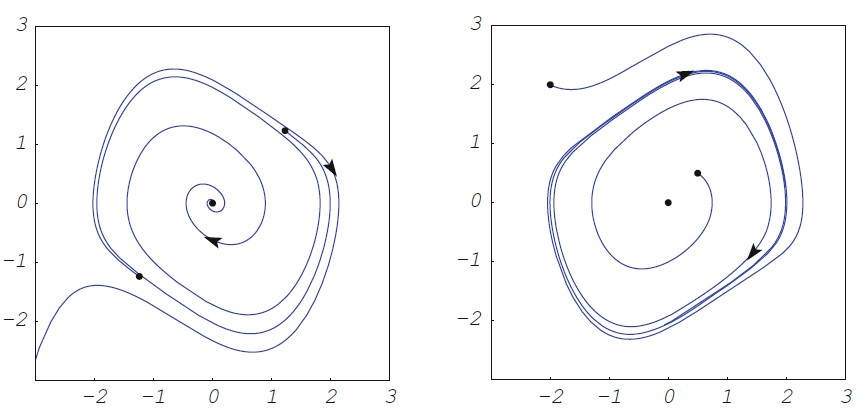
\includegraphics[scale=0.7]{Traiettorie}
\end{center}
Per valori di $\mu$ positivi, ovvero per cui si hanno delle traiettorie limite che attraggono i punti nello spazio delle fasi, si nota che l'ambiezza di queste curve cresce con lo smorzamento. \\
Come accennato in precedenza, nel caso particolare in cui $\mu = 0$, il sistema si riduce a un oscillatore armonico, quindi la traiettoria sarà una circonferenza.
\begin{center}
	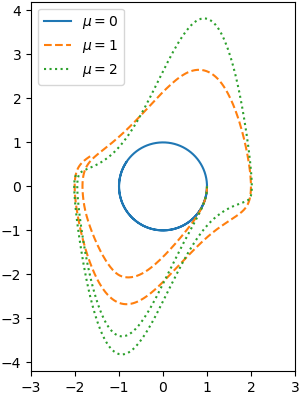
\includegraphics[scale=1]{Vari smorzamenti} 
\end{center}
\subsection{Storia}
L'oscillatore di Van Der Pol è stato ideato originariamente dall'ingegnere elettrico olandese Balthasar Van Der Pol. Van Der Pol scoprì delle oscillazioni stabili, che in seguito chiamò rilassamento-oscillazioni e che sono un tipo ci ciclo limite nei circuiti elettrici che utilizzano i vacuum tubes. \\

\subsection{Applicazioni}
\paragraph{Applicazioni ingegneristiche \\}
\paragraph{Il neurone \\}
\paragraph{Il modello di Fitzhugh-Nagumo \\}
\subsection{Varianti: L'oscillatore di Van Der Pol forzato}

\section{Soluzione numerica e simulazione}
Per risolvere l'equazione differenziale dell'oscillatore è stato scritto un codice in C++, che ha permesso di trovare i valori di $x$ per dei valori di tempo discretizzati $t = n\Delta$. Per fare ciò si è partiti dall'equazione 2, ma per permettere al computer di interpretarla la si è dovuta discretizzare, ottenendo il seguente sistema:
\begin{equation}
	\begin{cases}
	x_{n+1} = x_n + y_n\Delta \\
	y_{n+1} = y_n + \left(\mu(1-x_n^2)y_n - x_n\right)\Delta
	\end{cases}
\end{equation} 
Sulla base di questo sistema di equazioni discretizzate è stato quindi scritto il seguente codice: \\ \\ \\
Come di vede, questo codice prende come parametri di entrata le coordinate iniziali $x_0$ e $y_0$, il parametro di smorzamento $\mu$ e lo step temporale $\Delta$. L'ultimo parametro è il tempo $t$, e scegliendo questo valore si ottengono i valori della $x$ per ogni istante temporale precedente al $t$ scelto. \\
Mediante questo codice vogliamo osservare certe caratteristiche dell'oscillatore: \\
1) Vogliamo osservare la traiettoria caratteristica di un punto nello spazio delle fasi. \\
2) Vogliamo confrontare traiettorie diverse con stesse coordinate iniziali ma con diversi valori del parametro di smorzamento. \\
3) Vogliamo osservare un comportamento particolare del modello di Van Der Pol, ovvero che se prendiamo un insieme di tanti punti distribuiti in modo casuale nello spazio delle fasi, dopo poche iterazioni questi seguono tutti la stessa traiettoria, che è quindi una curva attrattrice. \\
4) Vogliamo infine osservare l'andamento temporale della posizione $x$ della particella. \\
Partiamo dal primo obiettivo, ovvero la traiettoria carattestistica: 
\begin{center}
	\begin{figure}[h]
		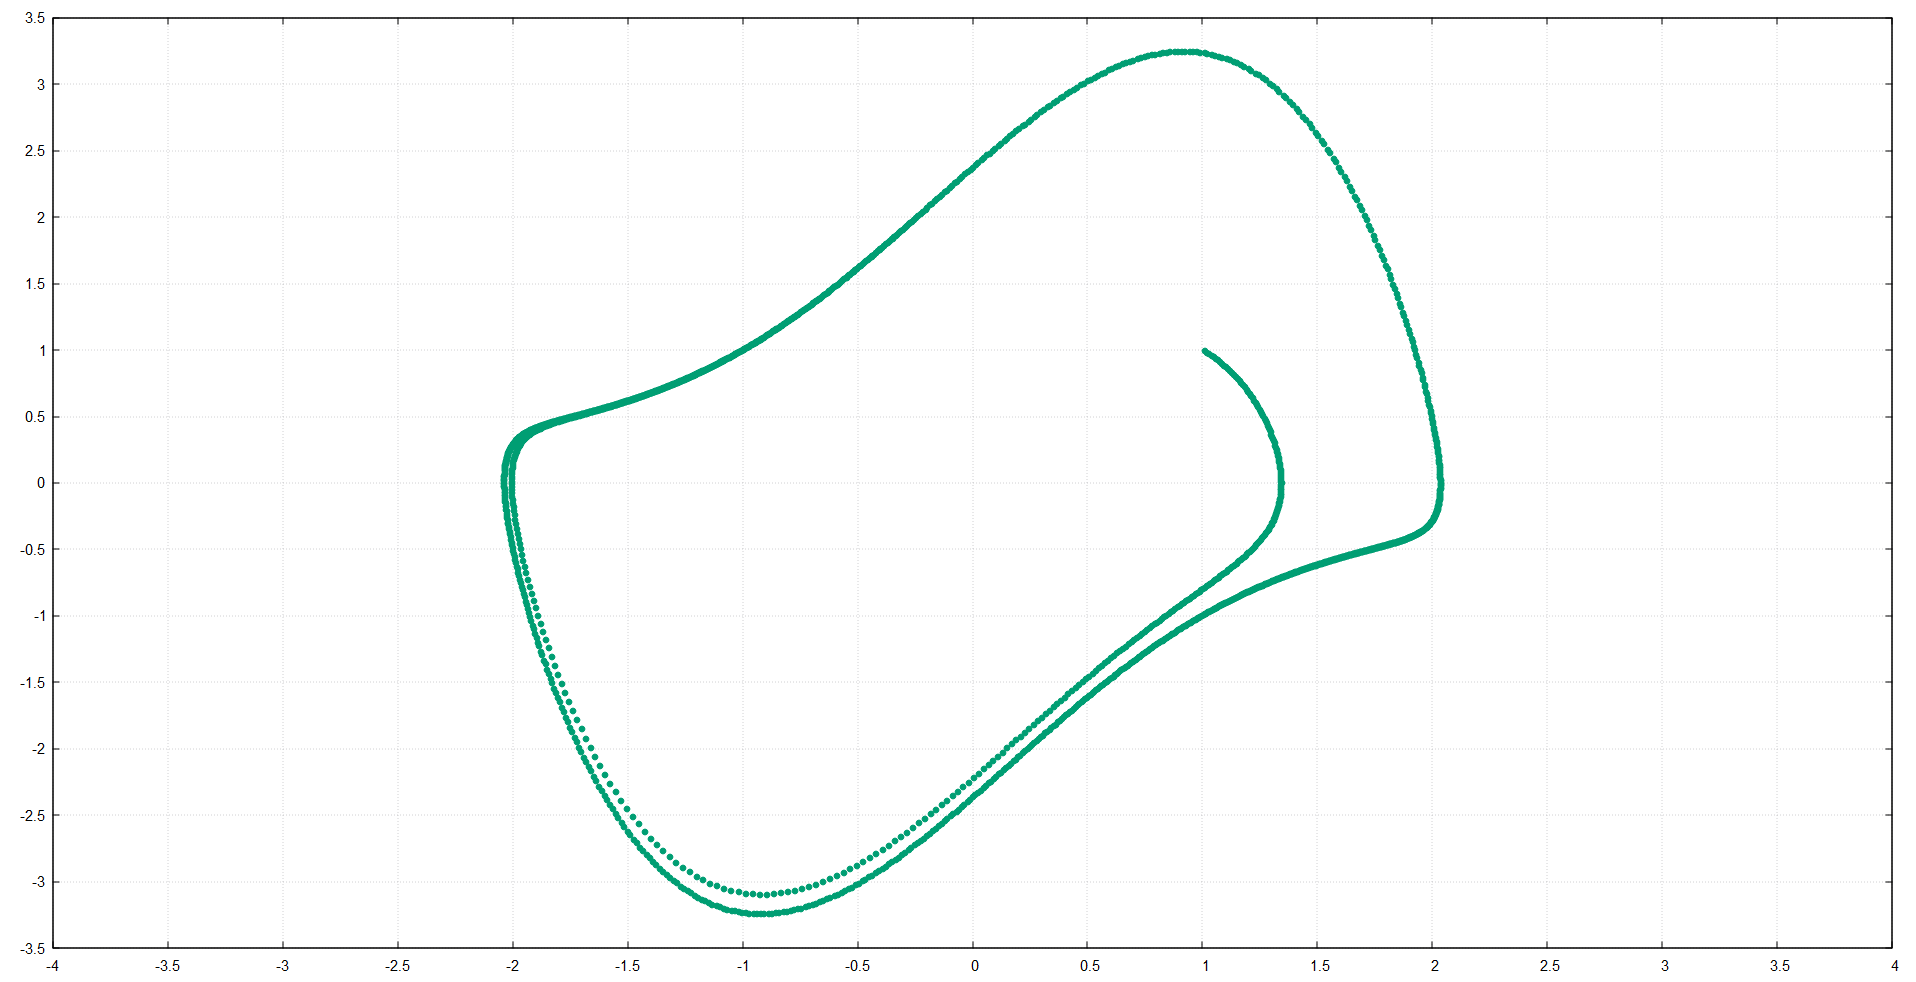
\includegraphics[scale=0.4]{mu1-5}
	\caption{Traiettoria nello spazio delle fasi di un oscillatore di Van Der Pol non forzato, smorzato con costante di smorzamento $\mu = 1.5$. L'asse orizzontale rappresenta la posizione mentre quello verticale rappresenta la quantità di moto.}
	\end{figure}
\end{center}
Nella figura soprastante si 
\begin{center}
	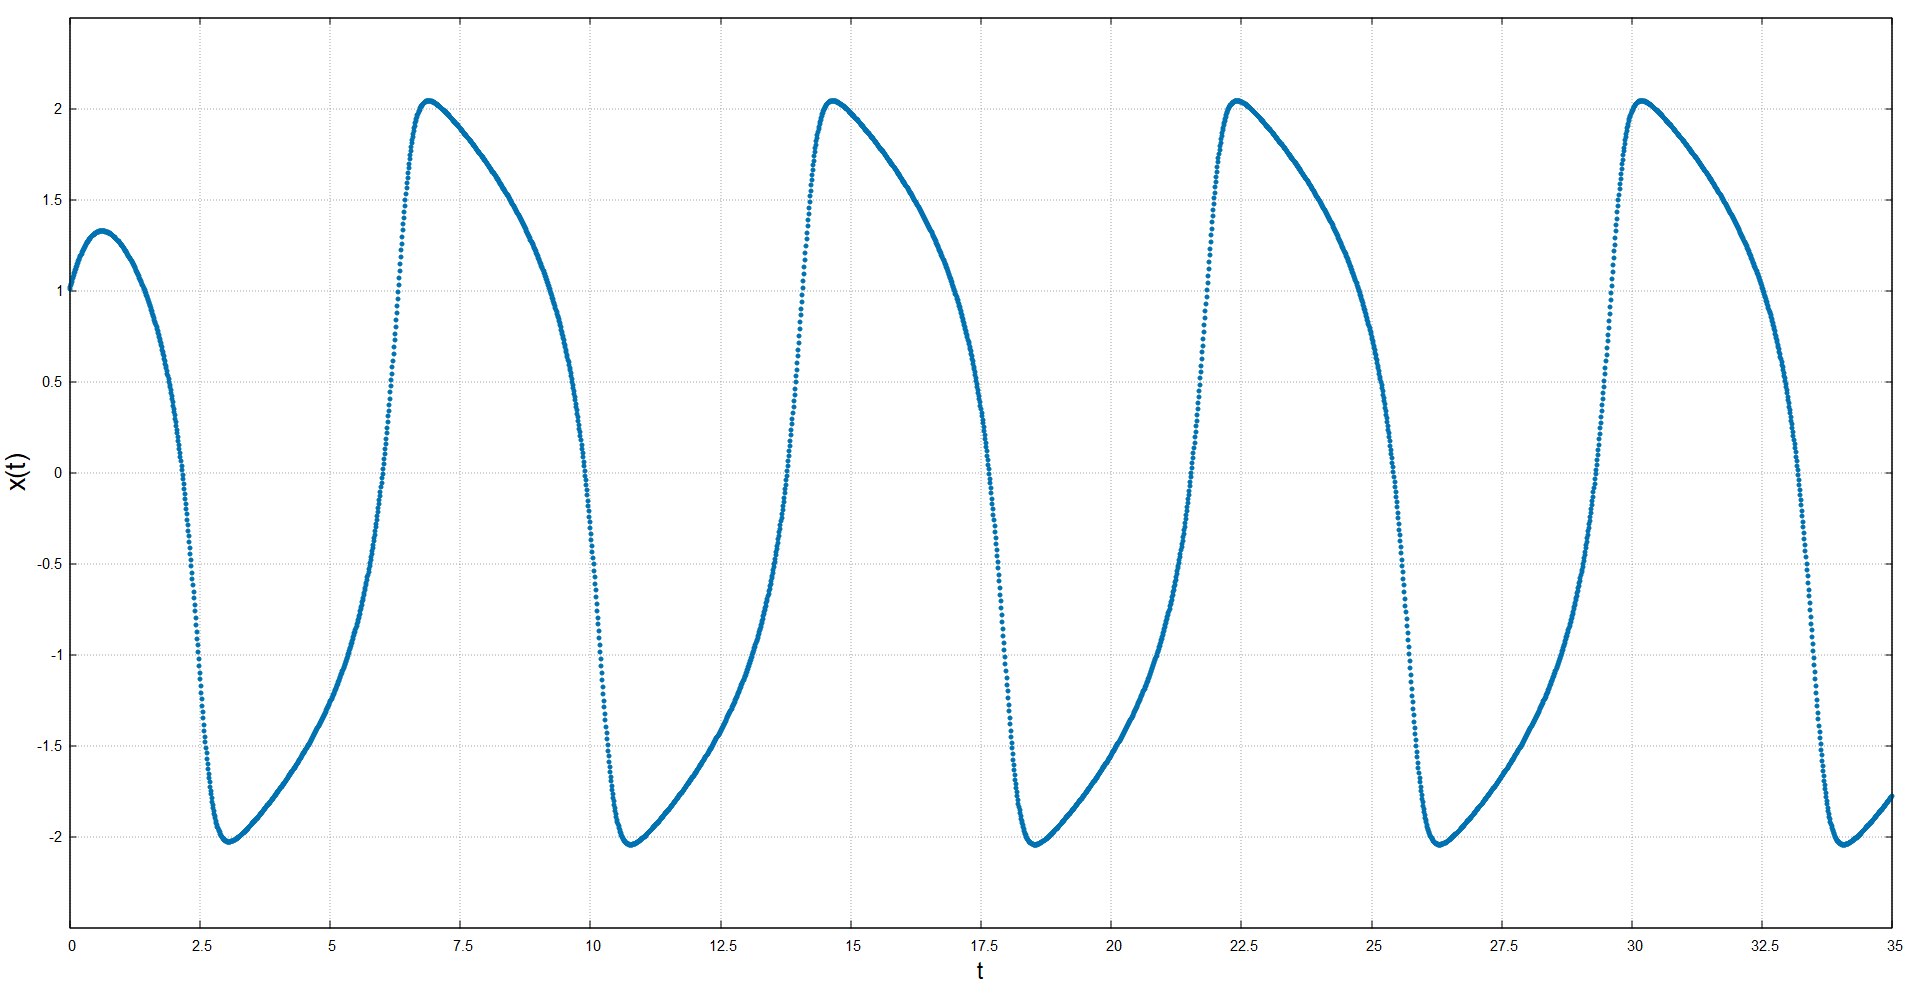
\includegraphics[scale=0.38]{Andamento temporale}
\end{center}

\begin{center}
	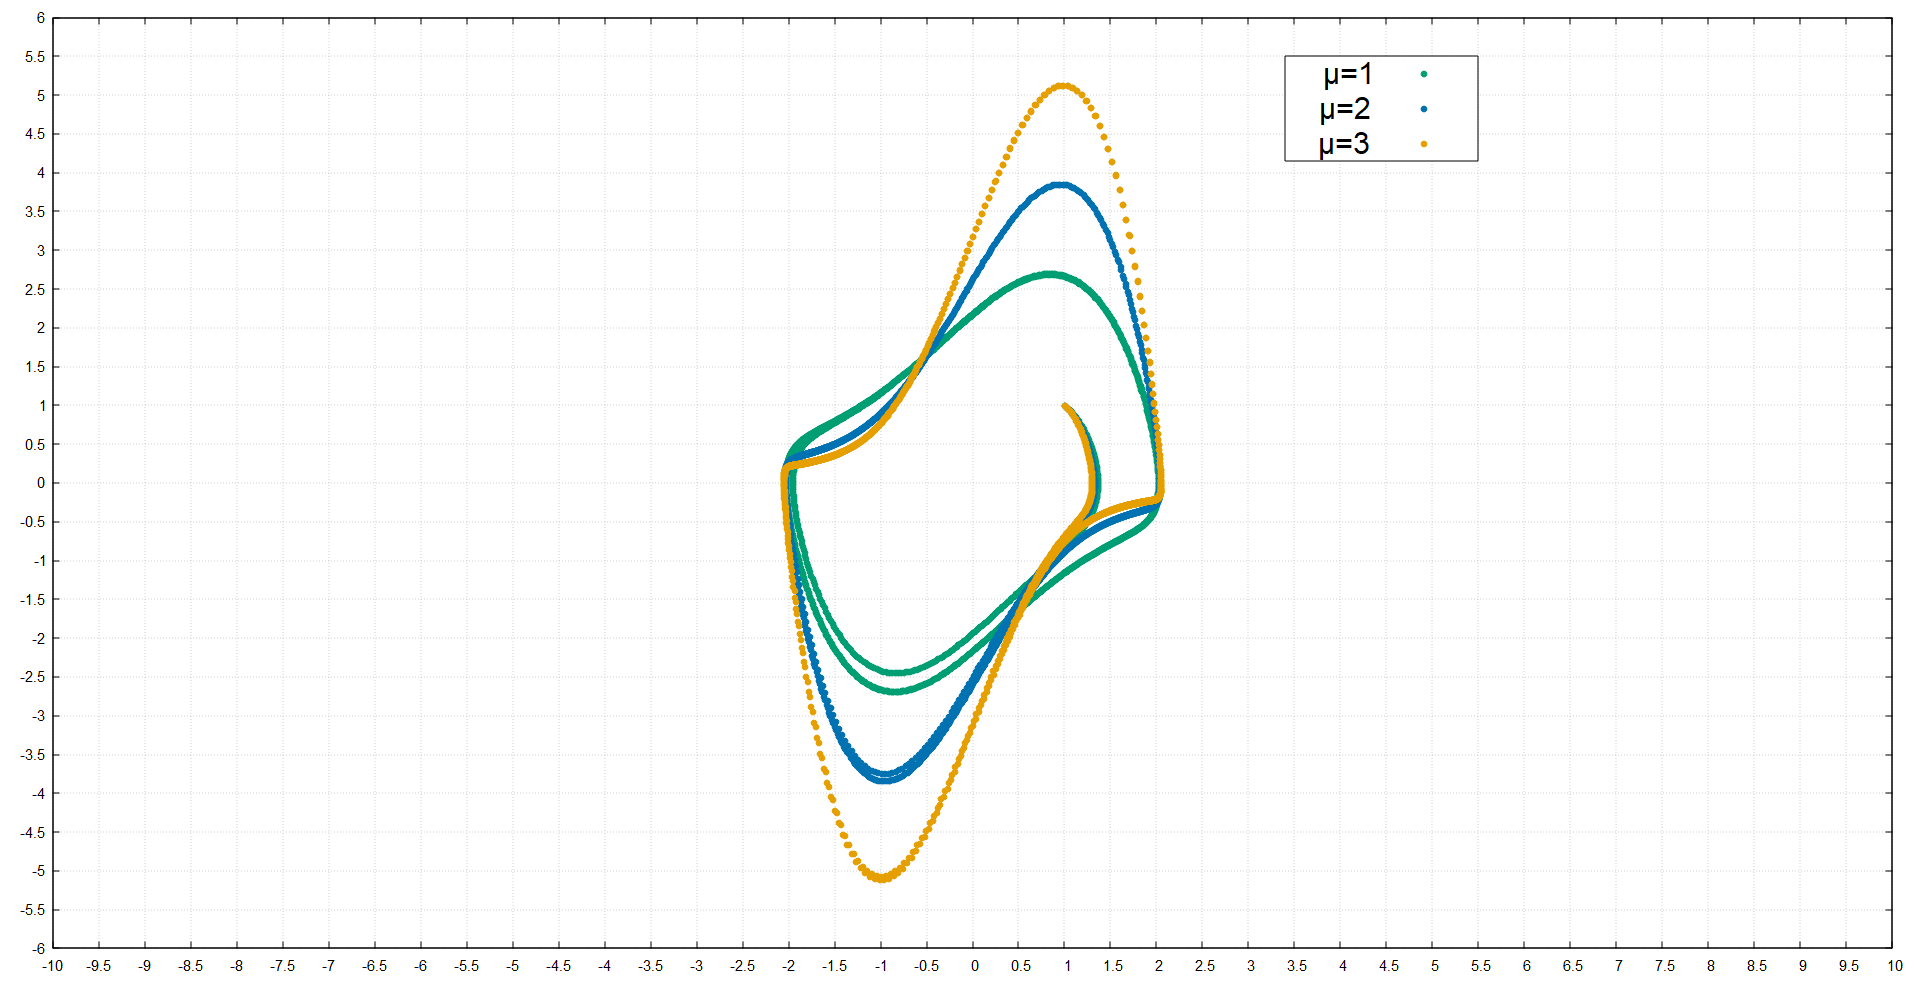
\includegraphics[scale=0.4]{mu123}
\end{center}
\section{Circuito elettronico}

\section{Trattazione hamiltoniana}


\end{document}